\documentclass{standalone}

\usepackage{graphicx,calc,epstopdf,tikz}

\graphicspath{{./figs/}}

\newlength{\tikzunit}
\setlength{\tikzunit}{\textwidth/16}
\newcommand{\compx}[1]{\textbf{#1}}

\begin{document}
\begin{tikzpicture}[scale=1, x=\tikzunit,y=\tikzunit]
    \node(0,0) {};
    \draw( 5.0, 5.0) node{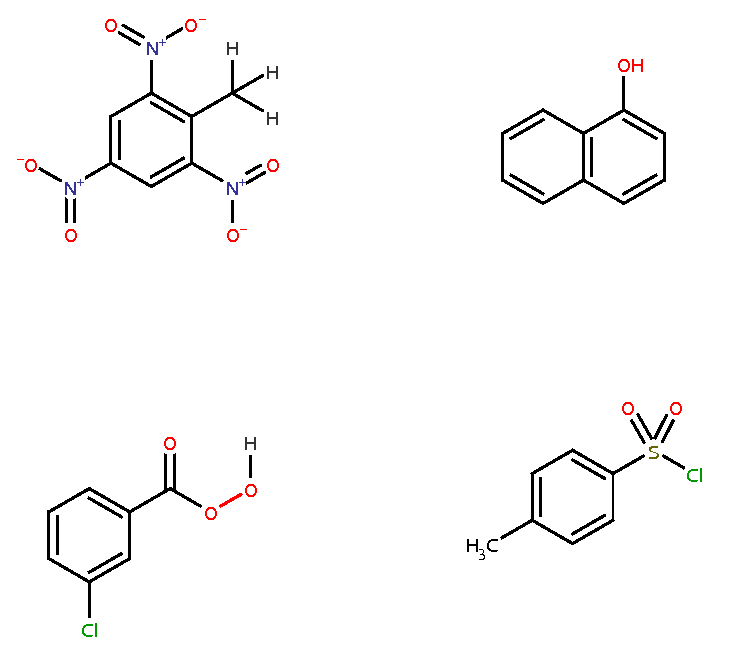
\includegraphics[width=9\tikzunit]{4struct.eps}};
    \draw(-5.0, 5.0) node{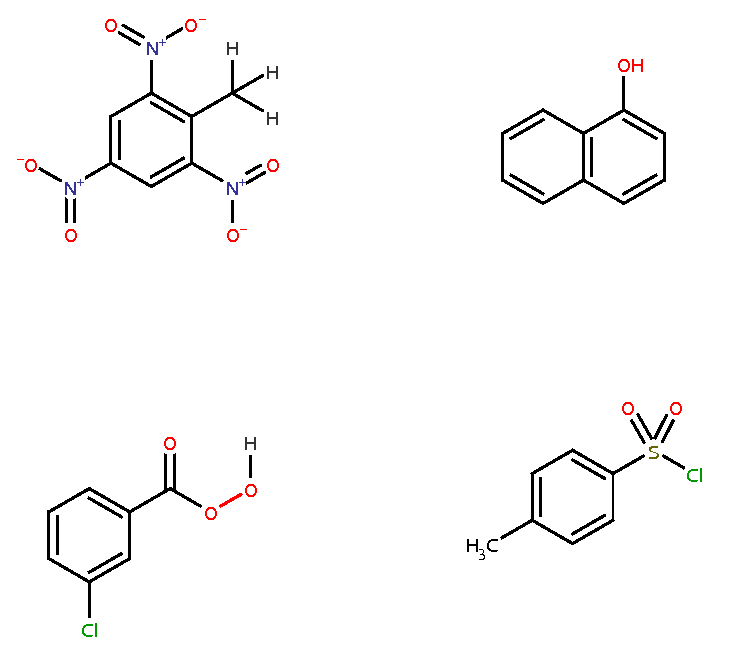
\includegraphics[width=9\tikzunit]{4struct.eps}};
    \draw( 5.0,-5.0) node{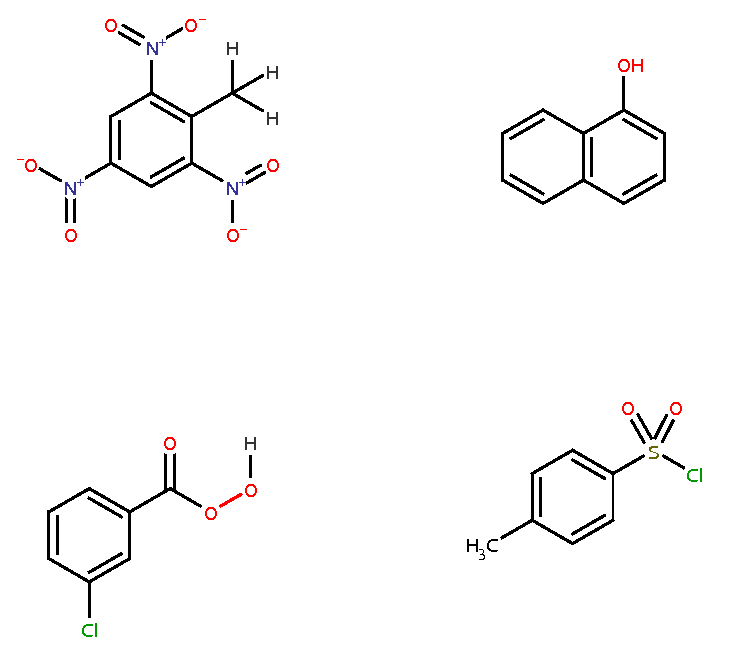
\includegraphics[width=9\tikzunit]{4struct.eps}};
    \draw(-5.0,-5.0) node{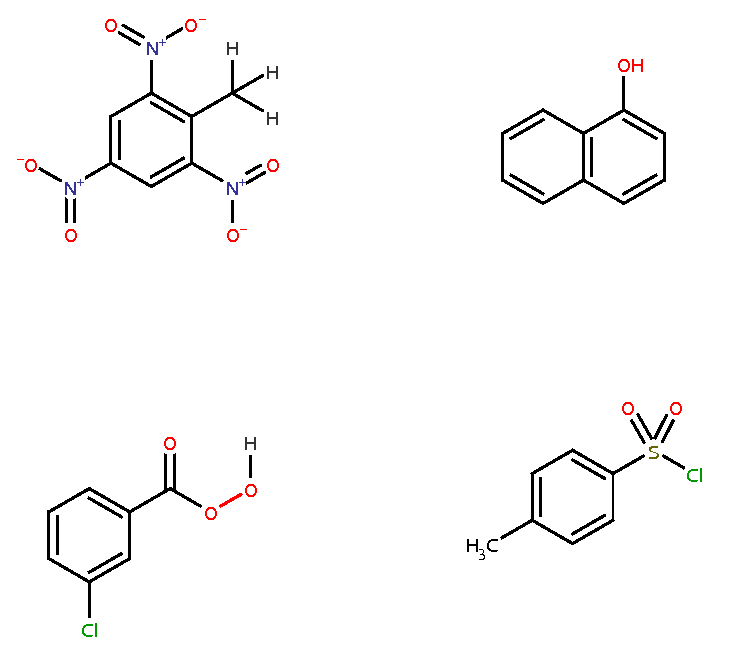
\includegraphics[width=9\tikzunit]{4struct.eps}};
    \draw(-9.8, 9.0) node[anchor=north west]{\textbf{a)}};
    \draw( 0.2, 9.0) node[anchor=north west]{\textbf{b)}};
    \draw(-9.8,-1.0) node[anchor=north west]{\textbf{c)}};
    \draw( 0.2,-1.0) node[anchor=north west]{\textbf{d)}};
    \draw[step= .20,color=gray,very thin] ( 0.05, 0.05) grid ( 9.95, 9.95);
    \draw[step=1.0,color=gray]            ( 0.05, 0.05) grid ( 9.95, 9.95);
    \draw[step=5.0,color=black]           ( 0.05, 0.05) grid ( 9.95, 9.95);
    \draw[step= .20,color=gray,very thin] (-9.95,-9.95) grid (-0.05,-0.05);
    \draw[step=1.0,color=gray]            (-9.95,-9.95) grid (-0.05,-0.05);
    \draw[step=5.0,color=black]           (-9.95,-9.95) grid (-0.05,-0.05);
    \draw (-7.8, -4.0) node{TNT};
    \draw ( 2.2, -4.0) node{TNT};
    \draw (-2.4, -4.0) node{Naphtol};
    \draw ( 7.6, -4.0) node{Naphtol};
    \draw (-7.8, -9.0) node{\compx{1}};
    \draw ( 2.2, -9.0) node{\compx{1}};
    \draw (-2.4, -9.0) node{\compx{2}};
    \draw ( 7.6, -9.0) node{\compx{2}};
\end{tikzpicture}
\end{document}
